\documentclass[a4paper,12pt]{article}
\usepackage{styles/iplouccfg}
\usepackage{styles/zhfontcfg}
\usepackage{styles/iplouclistings}

\graphicspath{{figures/}} 

\title{显著目标检测 --- 文献阅读}
\author{朱亚菲}
\date{2014年10月11日}

\begin{document}

\maketitle

\section{2007CVPR-Learning to Detect A Salient Object}

\begin{enumerate}
\item 基本思想

先对显著目标进行特征提取,得到多尺度对比度,中央-周围对比度,颜色空间分布3种feature maps,再用条件随机场模型进行组合,得到最终的显著性检测结果。

\item 方法流程
\begin{itemize}
\item Multi-scale contrast feature:本文将多尺度对比度特征$f_c(x,I)$定义为高斯图像金字塔中对比度的线性组合:
\begin{displaymath}
f_c(x,I)=\sum_{l=1}^L \sum_{x'\in N(x)}||I^l(x)-I^l(x')||^2
\end{displaymath}
其中$I^l$是高斯金字塔第l层图像,金字塔的层数L取6,N(x)为$9\times9$的窗。
\item Center-surround histogram:计算像素点$x'$为中心的显著矩形区域与其周围矩形区域的RGB颜色直方图之间的$\chi^2$距离;由于目标尺寸不同,选择不同纵横比的矩形区域进行测试,$\chi^2$距离最大对应得到最独特矩形区域;像素点$x$的中央-周围直方图特征定义为其所属所有矩形区域的空间高斯加权$\chi^2$距离之和。
\begin{displaymath}
f_h(x,I)\propto \sum_{\{x'|x\in R^*(x')\}} w_{xx'} \chi^2(R^*(x'),R^*_S(x'))
\end{displaymath}
\item Color spatial-distribution:图像中的所有颜色用高斯混合模型来表示,每一个像素被分配给具有某概率的颜色成分,计算每一个颜色成分的水平方差和垂直方差,得到该成分的空间方差;颜色空间分布特征定义为中央加权的 空间方差之和。颜色方差越小,该颜色越有可能属于显著目标。
\item 条件随机场结合:能量函数为K个显著特征和配对特征的线性组合,通 过条件随机场学习计算权重,得到最优化的线性组合。其中显著特征为前面 得到的3种feature map,用来描述一个像素点是否属于显著目标;配对特征为两个相邻像素点的空间关系,是对相邻像素标记为不同值的惩罚项。
\end{itemize}

\item 论文评价

采用条件随机场模型进行特征组合,融合颜色独立性,颜色空间分布和多尺度分布,考虑了局部信息,全局信息以及尺度信息。效果也不错。
\end{enumerate}

ITTI98论文主要提取亮度、颜色、方向三种特征,得到三种feature map。随后这些feature maps被归一化以便综合,综合方法是简单的相加。随后的很多研究都采取了这样的框架,针对特征提取/特征综合等等不同的阶段分别进行优化。
例如这篇:2006NIPS-Graph-based visual saliency.假定仍采用原先的特征提取方式,但是综合阶段使用的不是线性组合而是马尔科夫随机场,获得了比Itti更好的效果。本文采用条件随机场,与马尔可夫随机场相比,其优点是特征函数可以使用从整幅图像中提取的任意底层或高层特征。

\section{2008ICVS-Salient Region Detection and Segmentation}
这篇论文提出的算法的思想用其论文的一句话表达就是:

saliency is determined as the local contrast of an image region with respect to its neighborhood at various scales.

具体实现上,用这个公式表示:

\begin{displaymath}
c_{i,j}=D\left[\left(\frac{1}{N_1}\sum_{p=1}^{N_1} v_p\right),\left(\frac{1}{N_2}\sum_{q=1}^{N_2} v_q\right)\right]
\end{displaymath}

这里所说的尺度不是指改变图像的尺度而是改变R2区域的尺度,这样就可以得到全分辨率的显著图。

\lstinputlisting{Saliency_ICVS_2008.m}

关于这个算法的理论分析,FT算法那个论文里有这样一段话:

Objects that are smaller than a filter size are detected ompletely, while objects larger than a filter size are only artially detected (closer to edges). Smaller objects that are well detected by the smallest filter are detected by all three filters, while larger objects are only detected by the larger filters. Since the final saliency map is an average of the three feature maps (corresponding to detections of he three filters), small objects will almost always be better highlighted.

\section{2009CVPR-Frequency-tuned Salient Region Detection}

显著的区域和目标相比其周围背景会比较突出,本文的目的在于计算每个像素在颜色和亮度特征方面相对其领域的显著程度。大多数显著性检测方法都采用了相似的center-versus-surround方法,其中关键是看用来计算显著性的领域的尺度大小。本文将整幅图像看成是某一像素的领域。这也使得相对现在state-of-the-art的方法可以利用更多空间频率。

一般对图像进行滤波会导致只利用了原图的有限范围的频率信息来计算显著图,本文采用DoG(Difference of Gaussian)带通滤波器对图像进行滤波,即用两个尺度不同的高斯滤波器对原图像进行滤波后再相减。

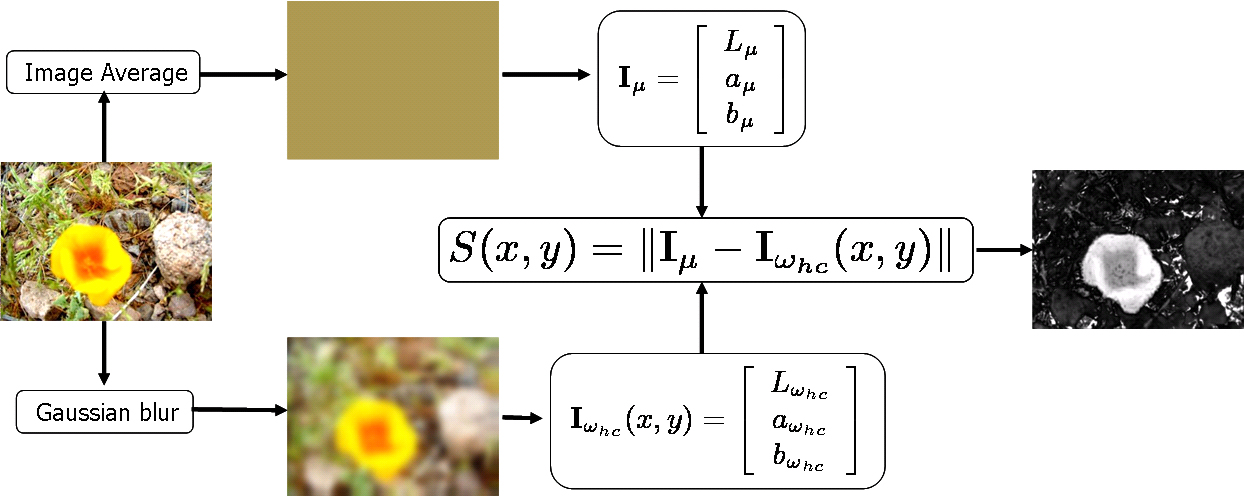
\includegraphics[width=\linewidth]{SaliencyAlgo.jpg}

这篇文章之后,很多工作的评价标准就从传统的对注视点预测的评价,转移到对物体区域二值图的预测上了。从某种意义上讲,这篇文章对Saliency detection的问题做了重新的定义,让问题定义更加回归实际应用。

\lstinputlisting{Saliency_CVPR2009.m}

\section{2014TPAMI-Global Contrast based Salient Region Detection}
本文在基于以下四点考虑的基础上,提出了提取高分辨率的全局显著性图像的分析方法:
\begin{itemize}
\item 基于全局对比度的方法倾向于将大范围的目标和周围环境分离开。这种方法要优于那些通常只在轮廓附近产生较高显著性的局部对比度方法。
\item 全局的考虑可以为图像中相似区域分配一个相近的显著性的值,并且可以均匀的突出目标。
\item 一个区域的显著性,主要是由它和周围区域的对比度决定,相距很远的区域起的作用较小。
\item 为了能够适应大规模图像集处理和高效的图像检索与分类的应用需求,显著图检测算法应该具有简单快速的特点。
\end{itemize}

1) HC:基于直方图对比度的方法,每一个像素的显著性值是由它与图像中所有其他像素的颜色差异来确定,得到全分辨率显著性图像;
\begin{displaymath}
S(I_k)=D(I_k,I_1)+D(I_k,I_2)+\ldots+D(I_k,I_N)
\end{displaymath}

2) RC:基于局部对比度的方法,先将图像分割成小区域,采用的分割方法是基于图的分割,基本分割思想是将每个像素点作为无向图的顶点,两个像素点之间的不相似度作为边的权重,要求连接相同区域内的两个顶点的边的最大权重要小于连接不同区域的顶点的边的最小权重,在迭代过程中进行顶点归纳与区域合并,具体参见论文Efficient graph-based image segmentation;每个区域的显著性值由它与其他所有区域的空间距离和区域像素数加权的颜色差异来确定;空间距离为两个区域重心的欧氏距离,较远区域分配较小权值;

3) 细节加速:

① 基于直方图的加速:将每个颜色通道由256个颜色值量化到12个颜色值后,对输入图像计算颜色直方图,保留高频颜色,覆盖95\%图像像素,剩下颜色舍弃,用直方图中距离最近的颜色代替;

② 颜色空间平滑:量化本身可能会有瑕疵,因为一些相似的颜色可能被量化为不同的值。为减小量化误差,每个颜色的显著性值被替换为相似颜色显著性的加权平均;在RGB空间进行量化,用Lab空间度量距离;

%4) 评价:基于HC的理论方法很简单,根据全局对比度计算显著度,计算速度快,对于背景较简单的图像效果也不错;RC改变了处理单元,由单个像素到图像块,速度较慢,效果并没有比HC提高很多,个人认为基于图的分割结果不够好,导致saliency map不均匀。

\section{2012CVPR-A Unified Approach to Salient Object Detection via Low Rank Matrix Recovery}

本文主要是做矩阵分解,根据论文Visual saliency detection via sparsity pursuit改进。

1、一幅图像可以表示成一个低秩矩阵与稀疏噪声的和,其中非显著的区域可以用低秩矩阵解释,而用稀疏噪声表示显著区域,本文不是第一次这样表示,在论文Visual saliency detection via sparsity pursuit中已采用过,其中,先将一幅图像通过uniformly sampling分解成8x8的patch,对每一个patch用超完备基进行稀疏编码,这些稀疏编码向量按列排列可形成一个矩阵。但这篇论文存在两个问题:(1)对于显著性检测而言,稀疏编码并不是非常好的特征表示方法,因为对于每个patch的稀疏编码是与噪声的稀疏性(显著性)无关的。经过uniformly sampling的patches仅仅由位置决定,有些sampled patches可能既包含背景又包含显著目标,因此不能保证背景矩阵一定是低秩的。(2)当显著目标较大时,这个显著目标内部可能被分成很多patch,可能两个patch对应的特征向量是相似的,这样用来表示显著性的噪声就可能不是稀疏的了。
  基于此,本文采用的方法是经过多尺度特征提取,并考虑空间信息,然后用mean-shift clustering方法将一幅图像分解成一些小区域(参照论文Mean shift: A robust approach toward feature space analysis)。每个区域中所有像素的特征向量的均值可看作其特征向量,将所有区域的特征向量按列排列可得到这幅图像的矩阵表示。这样改进的优点:(1)即使显著目标尺寸很大,其内部的区域分割数目也会很小,因为显著目标在空间位置和外观上都有连贯性。
(2)本文还通过标记数据训练得到一个线性特征变换来确保表示背景的矩阵在我们所学习的特征空间是低秩的。

2、论文Visual saliency detection via sparsity pursuit中用稀疏编码作来表示特征,本文用53个特征组成的特征向量来表示。

3、不是所有unique的区域都是显著的,因而需要高级先验知识来指导。在论文Context-aware saliency detection和论文Learning to predict where humans look中已经加入了这些高级先验知识,但其融合是对saliency map的后处理,也就是对由higher level cues产生的saliency maps与由low level features产生的saliency maps作加权平均,得到最终的saliency map。因而需要一种更有效的融合方法。

1) 基本流程:文章提出了一种新的图像表示方法,将其表示为一个低秩矩阵(非显著区域)加上稀疏噪音(显著区域),再利用Robust PCA技术进行低秩矩阵恢复,得到的噪音就是显著区域,再根据高层次的先验知识来帮助修正显著区域。

2) 图像矩阵:

 提取特征:R,G,B,hue,saturation,3尺度下4个方向共12个steerable pyramids响应,3尺度8方向共12个Gabor fileters响应,加起来一共53维。

 矩阵构造:先利用Mean-shift算法将图像分割成很多较小的segments再用每个segment中所有特征向量的均值来表示这个segment,从而构造成为矩阵。

 特征空间变换:保证特征向量为低秩。

3) 高层先验融合:位置先验(基于图像中心高斯分布),语义先验(人脸检测),颜色先验(暖色更明显)

%4) 评价:对图像的表示比较新颖,但实验效果一般,saliency map不均匀,提取特征多,计算量大,低秩矩阵恢复速度也比较慢

\end{document}
